\documentclass[../main]{subfiles}
\begin{document}
\section{Introduction}
    \label{sec:intro}
    Convolutional Neural Networks (CNNs) have enabled monumental progress in many computer vision tasks over the past five years, achieving and even surpassing human level cognition~\cite{szegedy2017inception,real2018regularized,hu2017squeeze}.
    Such networks are often carefully designed and have become very deep and large, especially the ones that claim to achieve state-of-the-art results.
    For example, the ImgaeNet Large Scale Visual Recognition Challenge (ILSVRC) for the year 2015 was won by a deep neural network from the ResNet~\cite{he2015deep} family with 152 layers and obtained a 3.57\% error rate.
    Unfortunately, very deep networks can have a large memory footprint and become slow during inference.
    While this may not be a big problem when the trained model is deployed as a cloud service, it becomes a deal breaker for deployments on to the vast majority of comparatively resource constrained mobile devices and embedded systems.
    
    Compressing trained CNNs has been suggested as one avenue to tame very large and deep networks for the purpose of deployment to resource constrained devices.
    While there has been significant progress in this direction recently (see the survey in~\cite{cheng2017survey}), it remains an active area of research with several open questions and challenges.
    One observation made in~\cite{cheng2017survey} is that the various approaches to compressing CNNs are somewhat orthogonal which raises the question ``What are the right principles to employ for compressing families of CNN model architectures?''
    Yet another question is whether smaller/shallower neural networks with faster inference can come (robustly) close to the state-of-the-art results achieved by the deep CNN families, and if this could be done without the trial and error overhead of hand designed model architectures.
    In this work, we pose and study three related questions:
    \begin{enumerate}
    	\item	For deploying models to resource constrained devices, the accuracy, memory footprint and inference speed of the deployed model are important considerations.
    	How do we control the trade-off between these quantities (henceforth, referred to as the `AMS trade-off')?
    	\item	In most applications, a deployed model will only see a reduced diversity of input data and/or will need to produce only a subset of the possible class labels.
    	Can this aspect be used to improve the AMS trade-off?
    	As a crude example, consider a neural network deployed on a self-driving car for identifying objects in its path.
    	Such a network might have been trained on the ImageNet dataset, but it only needs to be able to classify objects into two categories, viz. objects for which it needs to slow down or stop, and everything else.
    	\item	Current algorithms for model compression are fairly compute intensive.
    	Depending on the particular algorithm and the compression targets that need to be achieved, it could take anywhere from a few hours to a couple of days to get a satisfactory result.
    	If several different compressed models need to be generated, is it possible to reduce the amortized execution time?
    	As a real-world example, consider a deep neural network that needs to power the user experience on a mobile application.
    	Since users have different behavioral patterns, there is a case for deploying compressed models that are personalized to users/user segments.
    	Scaling such a `personalized compression' task beyond a few users becomes prohibitive very quickly.
    \end{enumerate}
    
    Our contributions are to help answer the above questions and we do so by developing an algorithm for compressing CNNs.
    We draw upon prior work in~\cite{ashok2017n2n} to utilize reinforcement learning (RL) to learn a compression policy for a given CNN trained on a given dataset, where compression is via architecture search and the reward function includes compression rate and accuracy of a candidate architecture (student model) trained using knowledge distillation~\cite{hinton2015distilling,romero2014fitnets} from the given CNN (teacher model).
    We name our method as Data-driven Compression (DDC) and add the following over and above the contributions in~\cite{ashok2017n2n}.
    \begin{enumerate}
	    \item	Besides compression rate and accuracy, we include inference time as a component of the reward function for RL.
	    Further, we design reward functions with user definable performance thresholds for each of the three metrics in the AMS trade-off.
	    The thresholds allow for control of the operating point in the AMS trade-off space for different deployment targets.
	    \item	We demonstrate that the compression policy learned on the full dataset generalizes to the compression task \wrt~data subsets having fewer class labels.
	    In other words, using the compression policy learned on the full dataset gives a \emph{better} AMS trade-off on the compression task \wrt~a data subset than executing the compression from scratch with a policy learned on the data subset.
	    Moreover, using the former compression policy leads to much faster completion (5x faster) of the compression task \wrt~data subsets than compressing from scratch.
	    This leads to much smaller amortized execution time as compared to other model compression algorithms when multiple compressed models need to be generated while maintaining an impressive AMS trade-off for each compressed model.
	    We conduct extensive experiments with ResNet and VGGnet model families trained on CIFAR datasets to demonstrate these results.
	    Finally, we note that the compression policy transfer claims and supporting experiments in~\cite{ashok2017n2n} are of an orthogonal nature.
	    Therein, it is claimed that the learned compression policy generalizes to the compression task on other models from the same architecture family, \eg~compression policy learned on ResNet-18 can generalize to compress ResNet-34 models.%
	   % \item  Training on subsets gives a better AMS trade-off for the task
    \end{enumerate}
    
    % \begin{figure}
    %   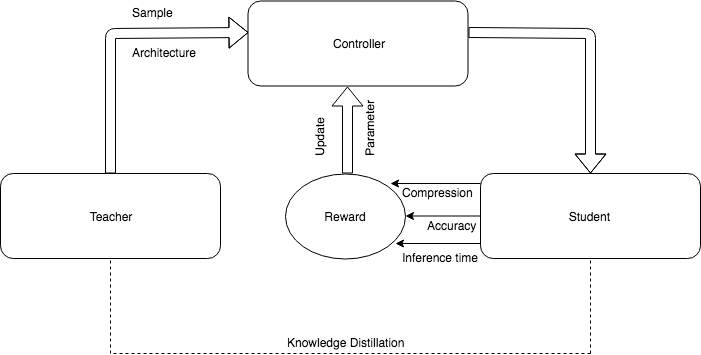
\includegraphics[width=\linewidth]{system}
    %   \caption{A recurrent controller which sample an architecture $p$ from the teacher model to produce a smaller student model.
    %   Combination of Accuracy $a$, Compression $c$ and Inference time $l$ is considered as a metric to scrutinize a generated architecture.
    %   This reward is then used to update the parameters of the recurrent controller.\hl{use draw.io to generate a better looking graphic in vector format}}
    %   \label{fig:boat1}
    % \end{figure}

%TODO: Finish paper outline if time permits.
%    The paper is organized as follows: Section~\ref{sec:related} provides an overview of the existing literature.
%    Section~\ref{sec:approach} gives the details of the proposed approach while Section~\ref{sec:expts} describes the experiments conducted to evaluate the approach.
%    Finally, Section~\ref{sec:conclude} concludes the paper.

\bibsubfile{named}{bibs/sub}
\end{document}
